En este capítulo se describe el proceso de análisis y procesado de los datos otorgados por la EMT.
Se ha dividido en tres etapas: \textbf{Limpieza y Preparación}, \textbf{Estudio y Gaussianidad} y \textbf{Preparación para Simulador}.


\section{Limpieza y preparación}
Esta sección detalla los distintos procedimientos seguidos en una primera fase iniciada tras la recepción
de los datos provenientes de la EMT. Podemos distinguir dos tipos de datos principalmente:
Datos Geoespaciales y Datos de Operación.



\subsection{Datos geoespaciales}
Estos datos se corresponden con elementos públicos obtenidos del \textbf{EMT Open Data Portal}\footnote{
\url{https://datos.emtmadrid.es/} (accedido: 9 de mayo de 2026)}, una iniciativa
de la entidad que busca reforzar su compromiso con la transparencia y la colaboración para la mejoría
en la gestión~\cite{balaguer2018}. Si bien el simulador no necesita la exacta localización de las 
paradas o de la ruta en cuestión, estos datos permiten una mejor visualización de cara a la construcción
del modelo. Además, guardan información del orden y código numérico de las paradas, por lo que
se impulsó su integración y tratamiento.


Dichos datos se encuentran en formato GeoJSON, un estándar dentro del ámbito geoespacial. No obstante,
debido a la ubicación de estos dentro de un fichero de extensión \enquote{CSV}, se encuentran
mal formateados, presentando comillas simples \enquote{' '} en vez de comillas dobles 
\enquote{\char`\"  "}, y juntando ambos sentidos de la ruta dentro de la misma celda.

Para subsanar esto, se recurre a un script de \textit{Python} encargado de modificar las celdas 
correspondientes a los datos geo, separando en dos ficheros distintos según sentido y cambiando las 
occurrencias de comillas simples por dobles. Por facilidad, además, se ramificaron según si se 
correspondian con referencias a la trayectoria de la línea, o a instancias de paradas. 
De esta forma, se obtienen de cada ruta cuatro archivos, dos por cada sentido, donde uno
contiene información de la topología de las uniones inter-parada, y el otro de los puntos referencia a 
las mismas.


Como se especifica con anterioridad, aparte de obtención y limpieza de los datos, por facilidad en La
implementación, estos pasaron por un proceso de transformación a formato \textit{ESRI shapefile}.
Para ello se usa la herramienta de código abierto \textbf{QGIS}. En la figura \ref{fig:qgis_converted}
se muestra como se visualizan los cuatro GeoJSON procesados y transformados a shapefile. Posteriormente,
en la figura \ref{fig:shapefile_gama} se muestran esos archivos shapefile ya dentro del
entorno de trabajo de la plataforma de agentes GAMA.



\begin{figure}[H]
 \centering
    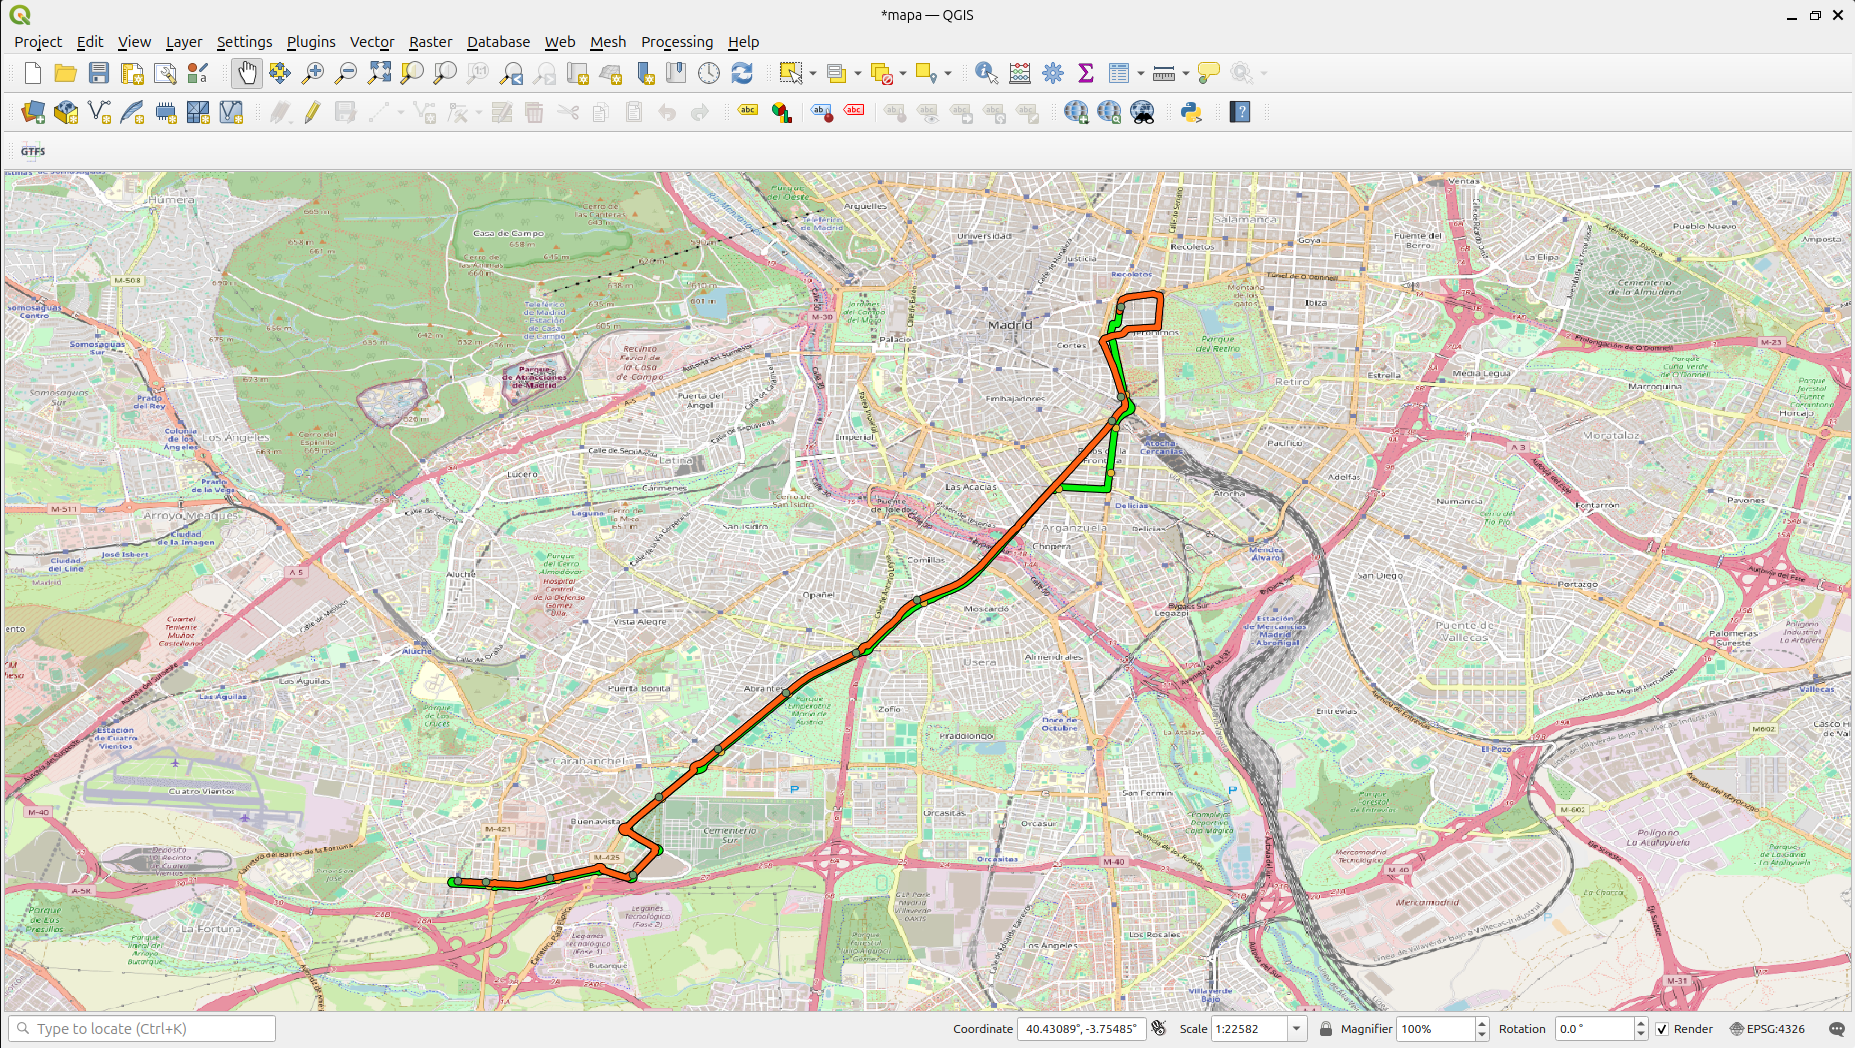
\includegraphics[width=\textwidth]{imagenes/qgis_capture_e01_converted.png}
\caption{Visualización en QGIS del mapa geoespacial convertido a shapefile}
\par\vspace{4pt}{\footnotesize Fuente: elaboración propia.}
\label{fig:qgis_converted}
\end{figure}


\begin{figure}[H]
 \centering
    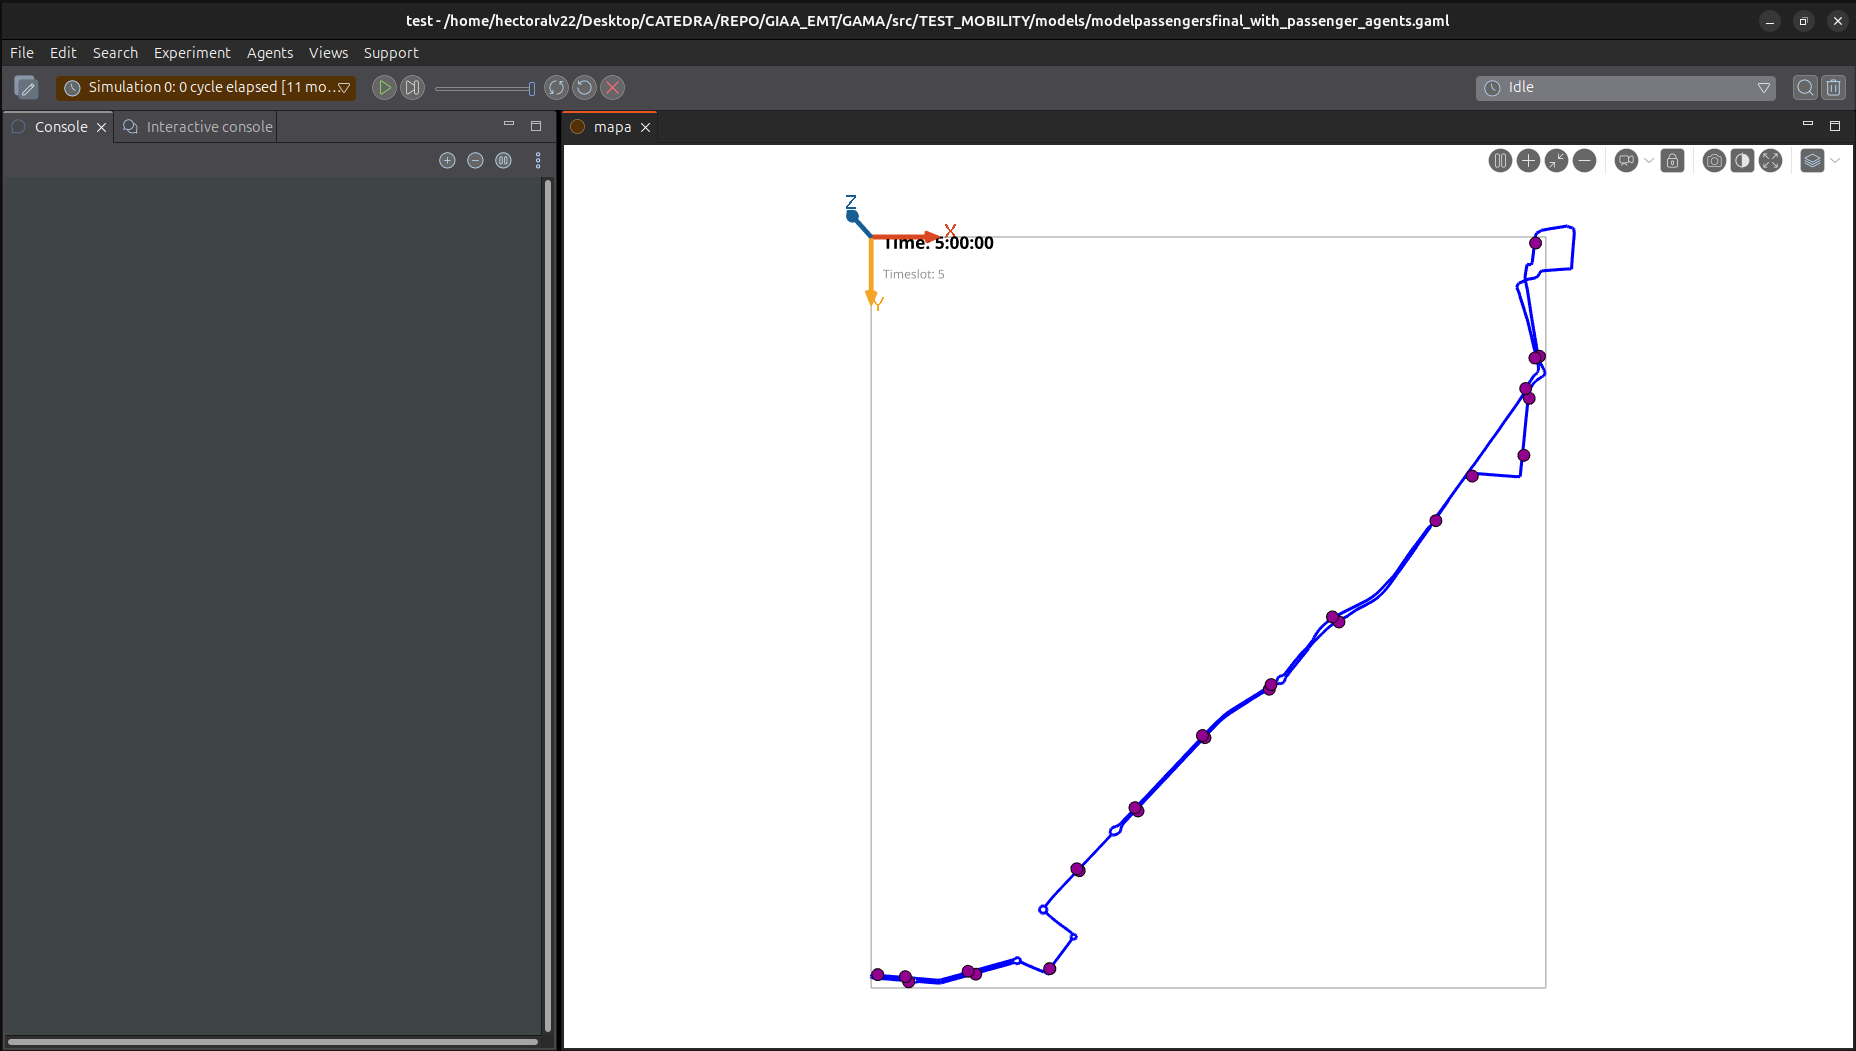
\includegraphics[width=\textwidth]{imagenes/gama_shapefiles.png}
\caption{Visualización en GAMA de los shapefile transformados}
\par\vspace{4pt}{\footnotesize Fuente: elaboración propia.}
\label{fig:shapefile_gama}
\end{figure}




\subsection{Datos de Operación}

Hablar de como se trabajaron los datos. Como se obtenian las tablas con  las consultas preparadas por stopcode, como se tuvo que limpiar valores negativos o anómalos, y explicar posibles discrepancias en primera y ultimas paradas debido(palabras de la emt quizas no se deba poner, que a veces los datos de inicio/fin estan falseados debido a que los conductores registran mal inicio/fin de viaje.

Los datos de operación representan la base empírica sobre la que se asienta el simulador.
Su tratamiento supuso el inicio formal de la fase dos del proyecto \textbf{Analisis y Parametrización},
debido a que la necesidad de la EMT  de preparar la base de datos en un servidor dedicado incluyendo el pipeline 
que alimenta diariamente los datos. Los geoespaciales por su parte, al ser de acceso público, se pueden tratar
sin la necesidad de preparación por parte de la empresa.

En la figura \ref{caption:relational_model} se puede ver el esquema relacional de la base de datos. Es un
modelo sencillo compuesto por dos tablas, Master y Transaccional, relacionadas por TripId,
identificador único de cada viaje. De esta forma, cada salida de cabecera representa una instancia de 
la tabla Master, mientras que cada llegada al resto de paradas de la ruta supone una entrada
de la tabla transaccional, identificada por el mismo TripId y el código de parada.


\begin{figure}[H]
 \centering
    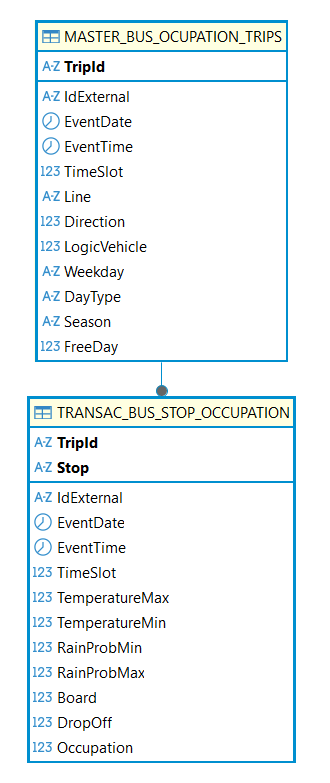
\includegraphics[width=0.5\textwidth]{imagenes/image_tables_diagram.png}
\caption{Modelo Master:Transaccional de la base de datos}
\par\vspace{4pt}{\footnotesize Fuente: Documento facilitado por la EMT.}
\label{caption:relational_model}
\end{figure}

\begin{lstlisting}[language=SQL, caption={Datos totales de una parada}]
SELECT mbot.*, tbso.*
FROM UCIII.Transport.MASTER_BUS_OCUPATION_TRIPS mbot
JOIN UCIII.Transport.TRANSAC_BUS_STOP_OCCUPATION tbso
    ON tbso.TripId = mbot.TripId
\end{lstlisting}
\par\vspace{4pt}{\footnotesize Fuente: Documento Facilitado por la EMT.}
